\documentclass[letterpaper,12pt]{article}
\usepackage{tabularx} % extra features for tabular environment
\usepackage{amsmath}  % improve math presentation

\usepackage{amssymb}

\usepackage{witharrows}
\usepackage{graphicx} % takes care of graphic including machinery
\usepackage[margin=1in,letterpaper]{geometry} % decreases margins
\usepackage{cite} % takes care of citations
\usepackage[final]{hyperref} % adds hyper links inside the generated pdf file
\hypersetup{
	colorlinks=true,       % false: boxed links; true: colored links
	linkcolor=blue,        % color of internal links
	citecolor=blue,        % color of links to bibliography
	filecolor=magenta,     % color of file links
	urlcolor=blue         
}
\usepackage{blindtext}
%++++++++++++++++++++++++++++++++++++++++


\begin{document}

\title{A look into a First Order Passive High Pass RC Filter}
\author{Dev Patel}
\date{\today}
\maketitle


In this short paper I'll dive into the passive, high pass RC Filters.



\section{What is a RC Filter?}

What is a RC Filter. A RC Filter is a filter circuit that uses only Resistors and Capacitors. RC Filters are used to adjust frequencies on circuits and have several applications in Signal Processing. An RC Filter is a type of Analog Filter. We will not explore Digital Filters in this paper.

RC Filters have something called a "cutoff frequency". This cutoff frequency determines the type of signal that can pass through the circuit. There are two types of RC Filters - High Pass, and Low Pass.

In a High Pass Filter, only Frequencies above the cutoff frequency are allowed. In a Low Pass Filter, only the Frequencies below the cutoff are allowed.

\section{ Passive High Pass Filter}

Before we get started exploring the High Pass Filter Theory, we need an example of what the Circuit would look like. In Figure 1, we have the basic circuitry for a 1st order High Pass Filter. Orders can Increase by adding more capacitors and resistors, similar to Figure 2.

\begin{figure}
    \centering
    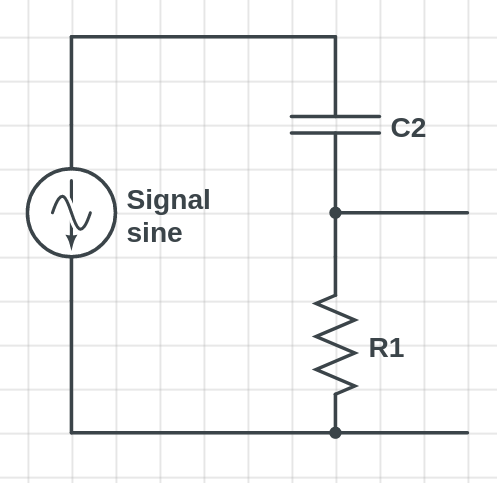
\includegraphics[width=30mm,scale=0.5]{highpassorder1.png}
    \caption{A basic example of a 1st order High Pass Filter}
\end{figure}
\begin{figure}
    \centering
    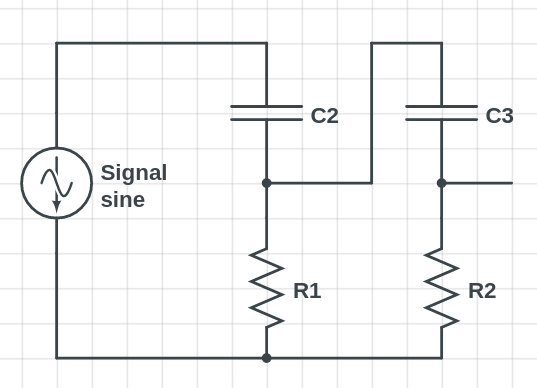
\includegraphics[width=50mm,scale=0.5]{highpassorder2.png}
    \caption{A basic example of a 2nd order High Pass Filter}
\end{figure}

The equation to solve for the cutoff frequency in a passive high pass filter is:
\begin{equation}
   F_c = \frac{1}{2\pi*RC}
   \label{Eq:frequencycut} %the label lets you refer to the equation later
\end{equation}
In the equation, F\textsubscript{c} represents the cutoff frequency. C represents the capacitance, and R represents the resistance.
Some values of F\textsubscript{c} that are used commonly are 40Hz for Music System Filters, and 150Hz for Voice System Filters.
Let's look at a Frequency Response Curve for a Passive High Pass Filter.
\begin{figure}
    \centering
    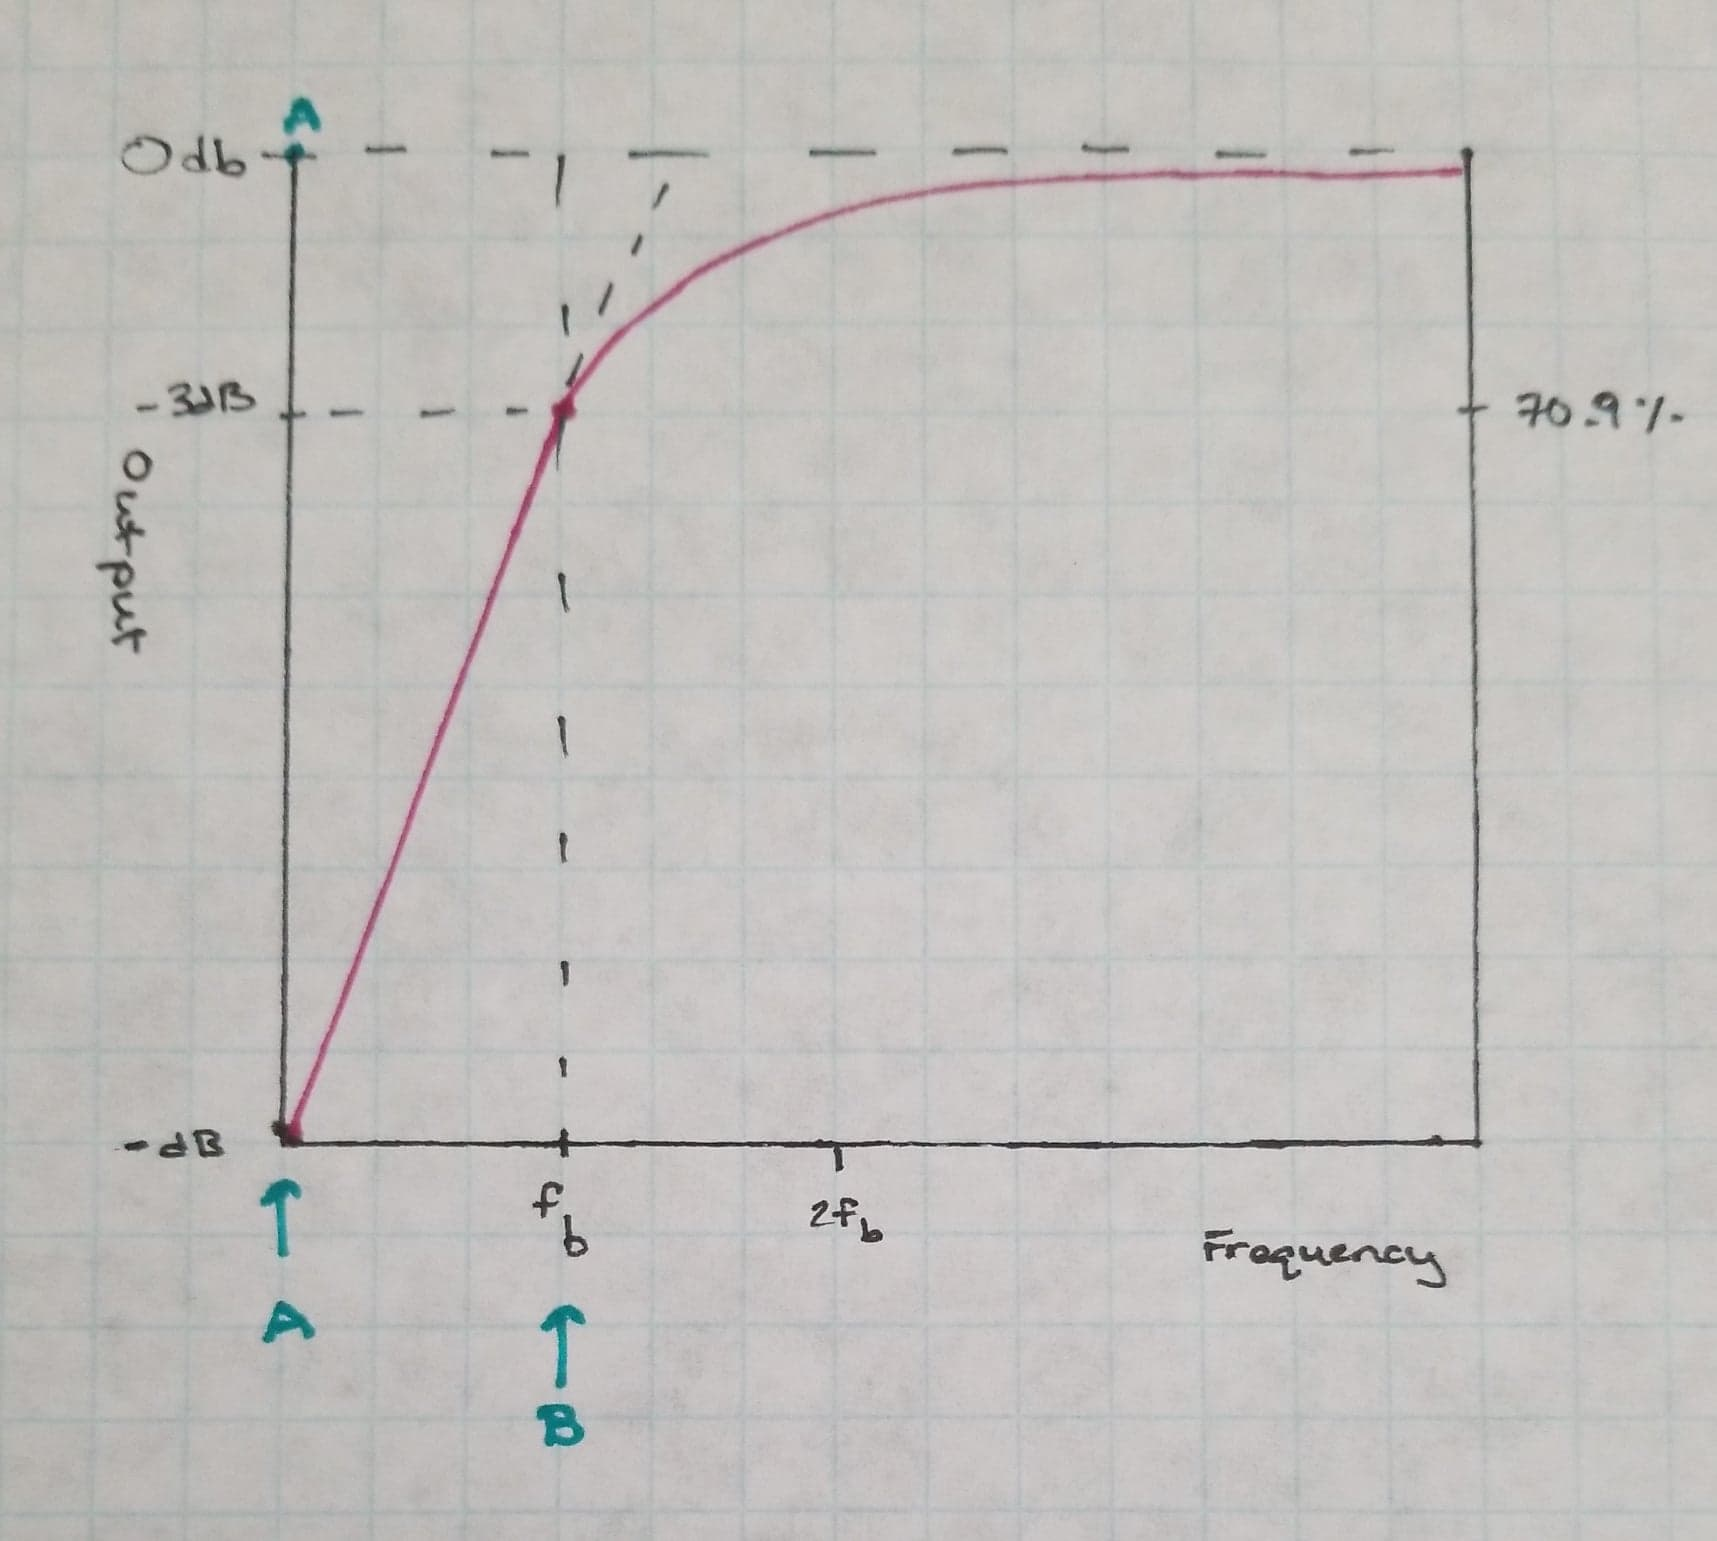
\includegraphics[width=60mm,scale=0.5]{bob.jpg}
    \caption{Frequency Response curve for a High Pass Filter}
\end{figure}
The Magenta line represents the frequency response curve. Point B on the curve is our frequency break point. The frequency break point always is about 3dB below the original signal, has a phase shift of about 45 degrees, and is where about 70.7\% of the signal goes through. The area on the graph from point A to B is called the \textbf{stopband}. The stopband is the area where the frequencies do not get past the filter. The area from B onwards to the right is the \textbf{passband} .

Let's take a deep dive into an example, 1st order passive high pass filter. The circuit schematics are the same as Figure 1. Our Sin signal has an amplitude of 1 volt, and has a frequency of about 150 Hz. We are going to select a resistance value of about 10k Ohms, which is recommended to use with 150Hz Signal. Now we can calculate our optimal capacitance value.

 \begin{equation}
    \setlength{\jot}{10pt}
    \begin{WithArrows}
    F_c = \frac{1}{2\pi*RC} \\
    CF_c= \frac{1}{2\pi*R} \\
    C= \frac{1}{2\pi*RF_c} \\
    C= \frac{1}{2\pi*10000*150} \\
    C=1.06*10^-7 farads\\
    \end{WithArrows}
    \nonumber
\end{equation}

Now that we have our capacitance value, we can now start to calculate $X_c$. $X_c$ is our capacitance reactance charge. $X_c$ will equal R at our breakpoint. We can mathematically verify this.
\begin{equation}
    \setlength{\jot}{10pt}
    X_c = \frac{1}{2\pi*CF_c} \\
    = \frac{1}{2\pi*1.06*10^-7*150} \\
    =10000 \Omega
    \nonumber
\end{equation}

Now that we have our $X_c$, R, C, and $F_c$, we can now mathematically justify why 70.7\% is retained at the breakpoint. To do that, we need to look into the phase shift. The phase shift of our curve at the breakpoint is 45 degrees. This would imply that both the X component (R) and the Y component ($X_c$) are the same (which is true at the breakpoint). So, lets use our 10K Ohms for R and $X_c$ as an example. \[\sqrt{10^2+10^2}\] is equal to about 14.1K. 10K/14.1K is about 70.7\%, which explains why at any breakpoint value in a passive, high pass filter, about 70.7\% of the signal passes through.



\section{Conclusions}
This has been a brief overview of the Passive High Pass Filter. Now go and create your own!



\end{document}
